% setup the document and include packages
\documentclass{article}[12pt]
\usepackage{amsmath}
\usepackage{amssymb}
\usepackage{cancel}
\usepackage{ntheorem}
\usepackage{graphicx}

% specify directories to find images
\graphicspath{ {./}{../scripts/png/} }

% redefine QED symbol
\renewcommand{\qedsymbol}{\rule{0.7em}{0.7em}}

% define lemma and result theorem-styled sections
\newtheorem{lemma}{Lemma}[section]
\newtheorem{result}{Result}[section]
\usepackage{easybmat}

% define shortcut for complex i
\newcommand{\iu}{{i\mkern1mu}}

% define subsubsection for homework
\renewcommand{\thesubsubsection}{\thesubsection.\alph{subsubsection}}

% define the title that will be used in the report
\title{CS 598 PS \\ Machine Learning for Signal Processing \\ Problem Set 1}
\author{
Christian Howard \\ howard28@illinois.edu
}
\date{} % don't set a date because we don't need this shit


% start the document
\begin{document}
   
   % create the title page 
   \maketitle
   \begin{abstract}
   Within this report, problems spanning probability, tensors, and signal processing were tackled and solved. To grab some extra credit, two sounds were recorded and were used to produce a spectrogram using the code created in the last problem. 
   \end{abstract}
   \newpage
   
   % create table of contents on separate page
   \tableofcontents
   \newpage
   
   % start section covering work on first problem
   \section{Problem 1 - A Probability Problem}
   For this first problem, the goal is to find the probability a woman has breast cancer given she has a positive mammograph. To present the solution to this problem, let me first define a few things that will prove useful. First, below is the notation for the various events:
   
   \vspace{10pt}
   \begin{tabular}{l l}
   $R_1$ = women has breast cancer & $R_2$ = women does not have breast cancer \\
   $M^{+}$ = mammogram is positive & $M^{-}$ = mammogram is negative
   \end{tabular}
   \vspace{10pt}   
   
   In the problem statement, we are given the following information:
   
   \begin{itemize}
   \item The probability that a woman has breast cancer is 0.8\%
   \item If a woman has breast cancer, there is a probability of 90\% that the mammogram will be positive
   \item If she has no breast cancer, the probability of a positive mammogram is 7\%
   \end{itemize}
   
   Based on the above information, we can find the following probabilities:
   
   \begin{align*}
   P(M^{+} | R_1) &= 0.9 \\
   P(M^{+} | R_2) &= 0.07 \\
   P(R_1) &= 0.008 \\
   P(R_2) &= 0.992
   \end{align*}
   
   Given the above information and definitions, our goal is to find $P(R_1 | M^{+})$. Using Baye's Rule, this becomes straight forward. The following is how we can arrive to the desired probability:
   
   \begin{align*}
   P(R_1 | M^{+}) &= \frac{P(M^{+} | R_1) P(R_1) }{P(M^{+})} \\
   &= \frac{P(M^{+} | R_1) P(R_1) }{P(M^{+} | R_1) P(R_1) + P(M^{+} | R_2) P(R_2)} \\
   &= \frac{(0.9) (0.008) }{(0.9) (0.008) + (0.07) (0.992)} \\
   &= 0.0939 \\
   &= 9.39\%
   \end{align*}
   
   Thus we find that the probability of a woman having breast cancer, given they got a positive mammogram, is 9.39\%.

	\newpage
	\section{Problem 2 - Manipulating Data using Linear Algebra}
	\subsection{}
	I am given $K$ grayscale images such that each image has dimension $M \times N$. For use as a data set, each image is vectorized and stuffed into a large data set matrix, $D$, that has dimension $(MN) \times K$.
	
	\subsubsection{}
	The goal for this part is to return the mean image, let us call it $\mu_I$, for the above data set and return it as an $M \times N$ matrix. 
	
	Given the data set is represented by the matrix $D$, one can multiply $D$ by a vector that will do the averaging for the vectorized form of the images and then invert the vectorization of the result. This final operation can be defined as the following:
	
	\begin{align*}
	\mu_I &= (D \boldsymbol{v} )^{(M)}
	\end{align*}
	
	where $\boldsymbol{v} = (v_1, v_2, \cdots, v_{T})$ is defined such that $v_i = \frac{1}{K} \forall i$ and $T = MN$.
	
	\subsubsection{}
	The goal for this part is to compute a $2 \times 2$ covariance matrix where this covariance is based on the mean color for the top and bottom half of a given image for all $K$ images in the data set. 
	
	Based on looking at patterns with simple $D$ values, a transformation was found for going from a vectorized image to a two element vector with the two half image averages we desire. For notational simplicity, let us define $I_p$ as an identity matrix of size $p \times p$. Using this definition, the transformation matrix can be defined like so:
	
	\begin{align*}
	H_{(M,N)} = \boldsymbol{1}_{(N)}^{T} \otimes I_2 \otimes \left( \frac{2}{M} \boldsymbol{1}_{(M/2)}^{T}\right)
	\end{align*}
	
	where $\boldsymbol{1}_{(p)} \in \{1 \}^{p \times 1}$ (i.e. a column vector of $1$s of dimension $p$). Using this matrix, and using the same $\boldsymbol{v}$ from the last problem, we can compute the covariance $\Sigma$ using the following:
	
	\begin{align*}
	D_{\mu} &= H_{(M,N)}D \\
	\boldsymbol{\mu} &= D_{\mu} \boldsymbol{v} \\
	\boldsymbol{\delta} &= D_{\mu} - \boldsymbol{1}_{(K)}^{T} \otimes \boldsymbol{\mu} \\
	\Sigma &= \frac{1}{K-1} \boldsymbol{\delta} \boldsymbol{\delta}^{T}
	\end{align*}
	
	\subsection{}
	To make things more interesting, now we are given a set of $K$ colored images where this whole data set is represented as a $M \times N \times 3 \times K$ tensor called $D$, where the dimension of size 3 is the color channel dimension.
	
	\subsubsection{}
	For this part we are asked to compute the average image across both the $K$ data samples and $3$ color channels, which I will define as $\mu_I$. First, for notational simplicity, let us define $I_p$ as an identity matrix of size $p \times p$. With this, we can find an operator to find the average image in its vectorized form using the following operation:
	
	\begin{align*}
	\mu_I &= \left(\left(\frac{1}{K}\boldsymbol{1}_{(K)}^{T} \otimes \frac{1}{3} \boldsymbol{1}_{(3)}^{T} \otimes I_N \otimes I_M\right) \text{vec}(D) \right)^{(M)}
	\end{align*}
	
	Working left to right in the Kronecker product sequence, the first term represents an averaging row vector over the $K$ pieces of data. The second term from the left then specifies an averaging row vector over the $3$ color channels. This vector then undergoes a Kronecker product with a sequence of identity matrices of dimensions $N \times N$, and $M \times M$ going from left to right. The resulting matrix, after all the Kronecker products, will take the vectorized data set and produce an $M \times N$ average image $\mu_I$.
	
	\subsubsection{}
	This next part is to instead compute the average image within just the red channel of the matrix. We will keep in mind that since the image is RGB, red will be the first channel in the third tensor dimension. With this defined, we can find the average $M \times N$ red channel image, $\mu_r$,  using the below operation:
	
	\begin{align*}
	\mu_r &= \left( \left(\frac{1}{K}\boldsymbol{1}_{(K)}^{T} \otimes [1,0,0] \otimes I_N \otimes I_M\right) \text{vec}(D) \right)^{(M)}
	\end{align*}

Using the above operation, the second term $[1, 0, 0]$ effectively zeros out contributions from the green and blue channels, producing an average vectorized $M \times N$ image which represents the average red channel image. We then vec-transpose the result to obtain an $M \times N$ average red image.

\newpage
\section{Problem 3 - Signal Processing is Linear Algebra}
Within this problem, the goal is to find an expression for a matrix $A$ such that one can multiply this matrix by some input sound $\boldsymbol{x}$ and produce the vectorized complex-valued spectrogram for this sound. Some desired traits for this matrix $A$ are the following:

\begin{itemize}
\item The transformation will be based on a 1024 point Discrete Fourier Transform (DFT)
\item The transformation will use a Hann window
\item The transformation will be based on a hop size of 512 points
\end{itemize}

For notational convenience, let us define $N$ as the number of points having the windowing and DFT performed on them. Let us also define $h$ as the hop size value being used and $M$ as the number of windows we will be processing. To formulate this matrix $A$, let us first take a look at a local window of $N$ data points. The transformation needed to process this data is the matrix $B$, defined below as:

\begin{align*}
B = DH
\end{align*}

where $D \in \mathbb{C}^{N \times N}$ is the Fourier Matrix defined as $D_{jk} = \frac{1}{\sqrt{N}}e^{2\pi \iu j k /N  }$ and $H = \text{diag}(\boldsymbol{w})$ where $\boldsymbol{w} = [w_0, \cdots, w_{N-1}]^{T}$ and the elements of $\boldsymbol{w}$ can be defined as:

\begin{align*}
w_k = \frac{1}{2} \left( 1 - \cos\left(\frac{2 \pi k}{N-1}\right)\right)
\end{align*}

\newpage
Given the definition of matrix $B$, we can then construct the overall matrix $A$ by embedding $B$ within $A$ as $M$ different submatrices shifted $h$ columns to the right and $N$ rows down relative to where the previous submatrix is located. This can be visualized by using the structure shown below:

\begin{figure}[h]
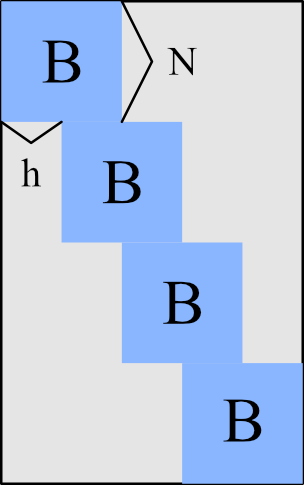
\includegraphics[scale=0.4]{block_matrix}
\centering
\end{figure}

Using this structure, an example graphic of $||A||$ with the DFT and Hann window built into it is the following:

\begin{figure}[h]
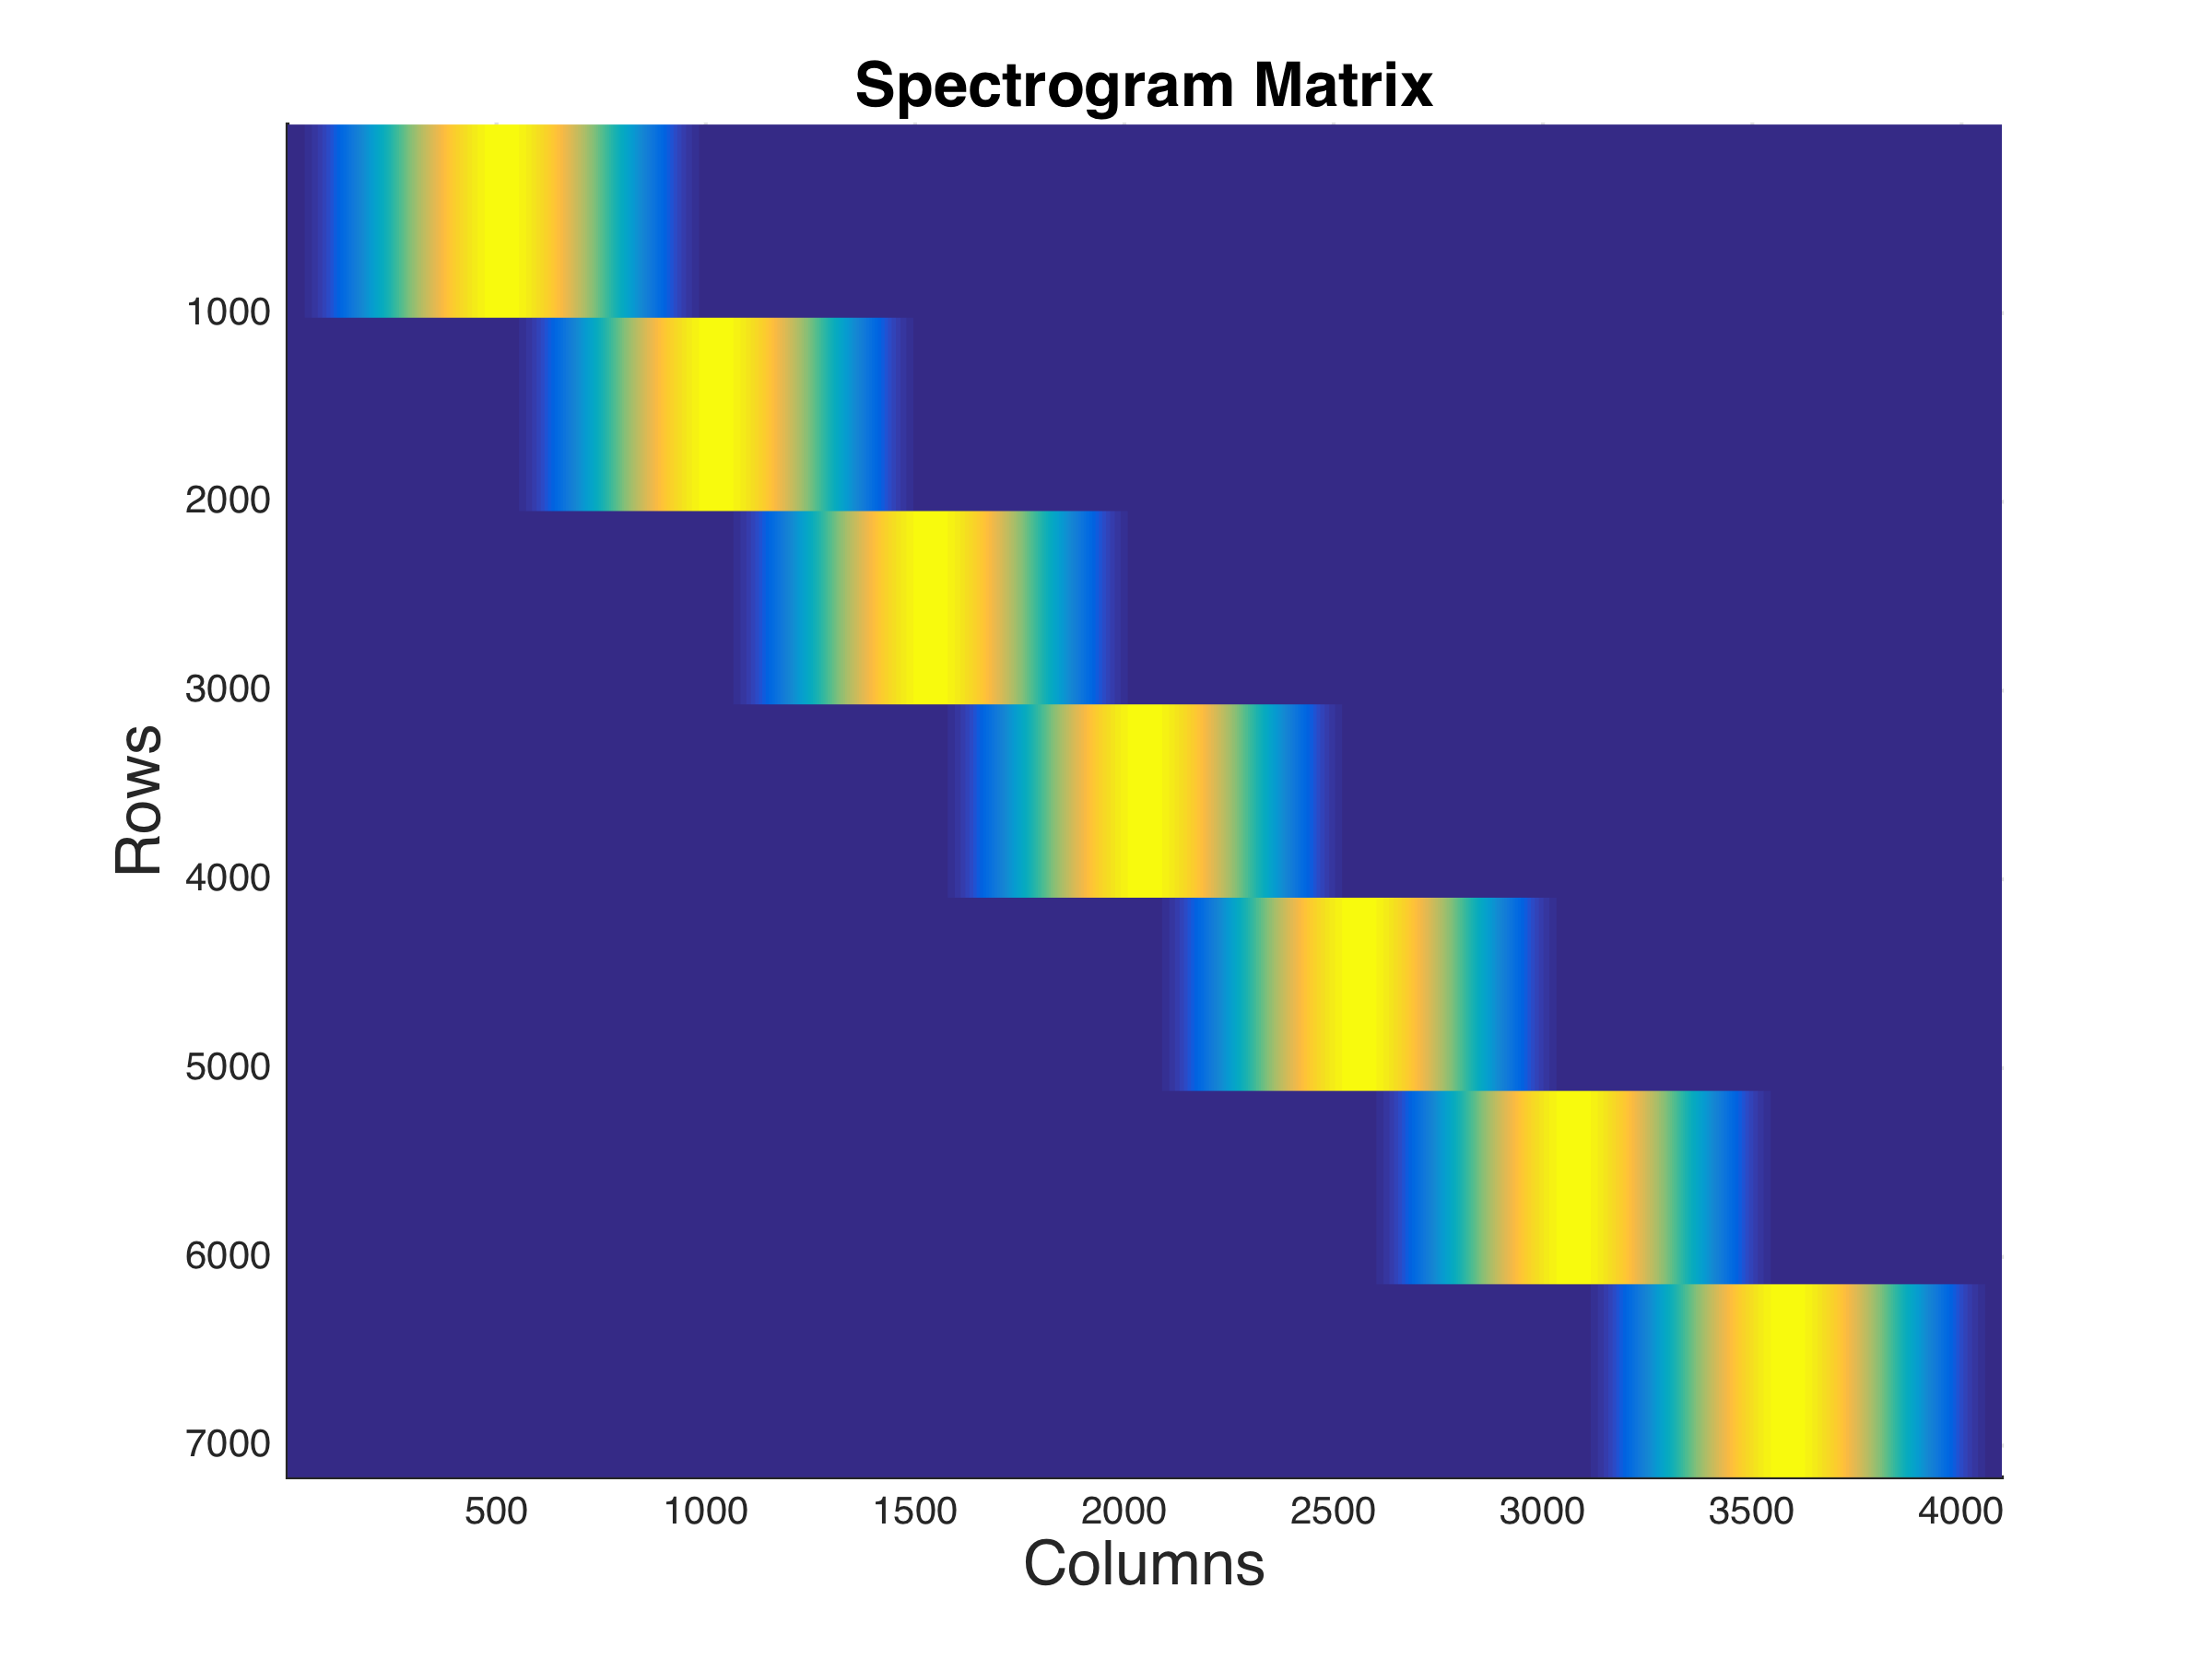
\includegraphics[scale=0.35]{spectrogram_matrix}
\centering
\end{figure}

Now with matrix $A$ defined properly, we can then produce a $N \times M$ spectrogram matrix $S$ using the following:

\begin{align*}
S &= (A \boldsymbol{x})^{(N)}
\end{align*}

\newpage
Using this formulation for $A$ and the specific constraints mentioned above, i.e. $N = 1024$, $h = 512$, below are two sample spectrograms based on two sounds that I recorded so I can grab some of that extra credit:

\begin{figure}[h]
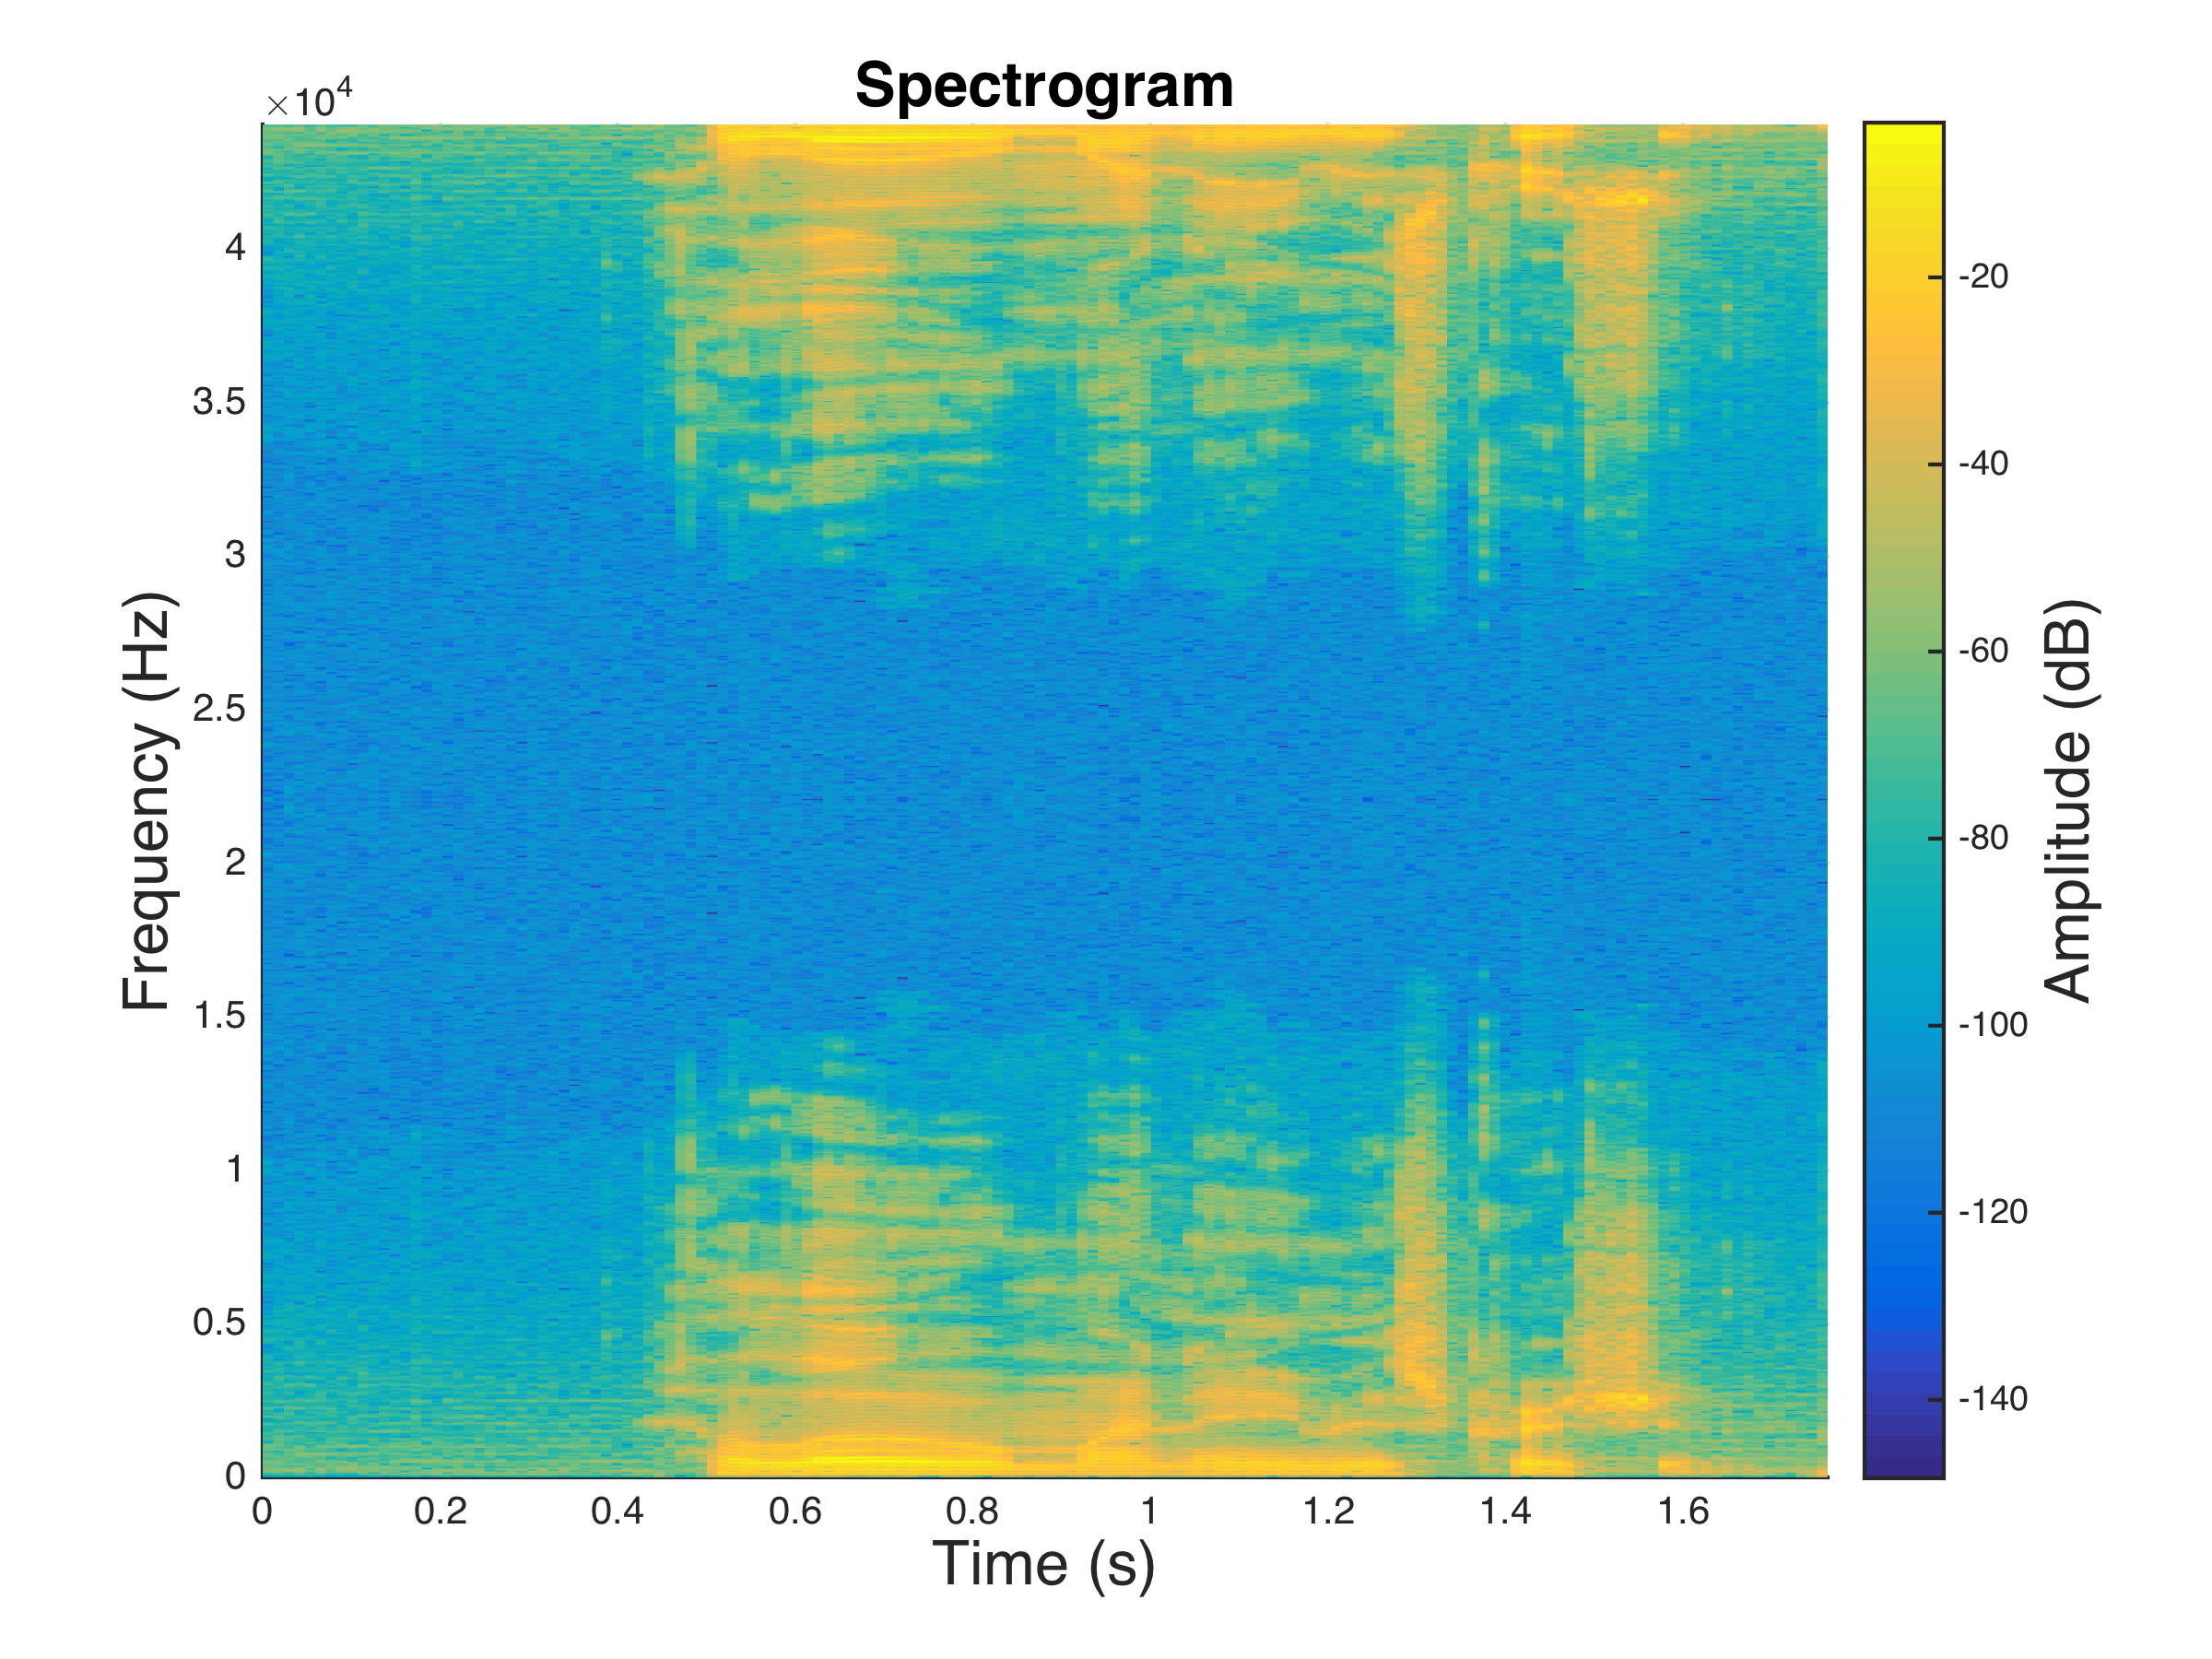
\includegraphics[scale=0.35]{hello_clip2_spectrogram}
\centering
\caption{Spectrogram from saying "Hello my name is Christian"}
\centering
\end{figure}

\begin{figure}[h]
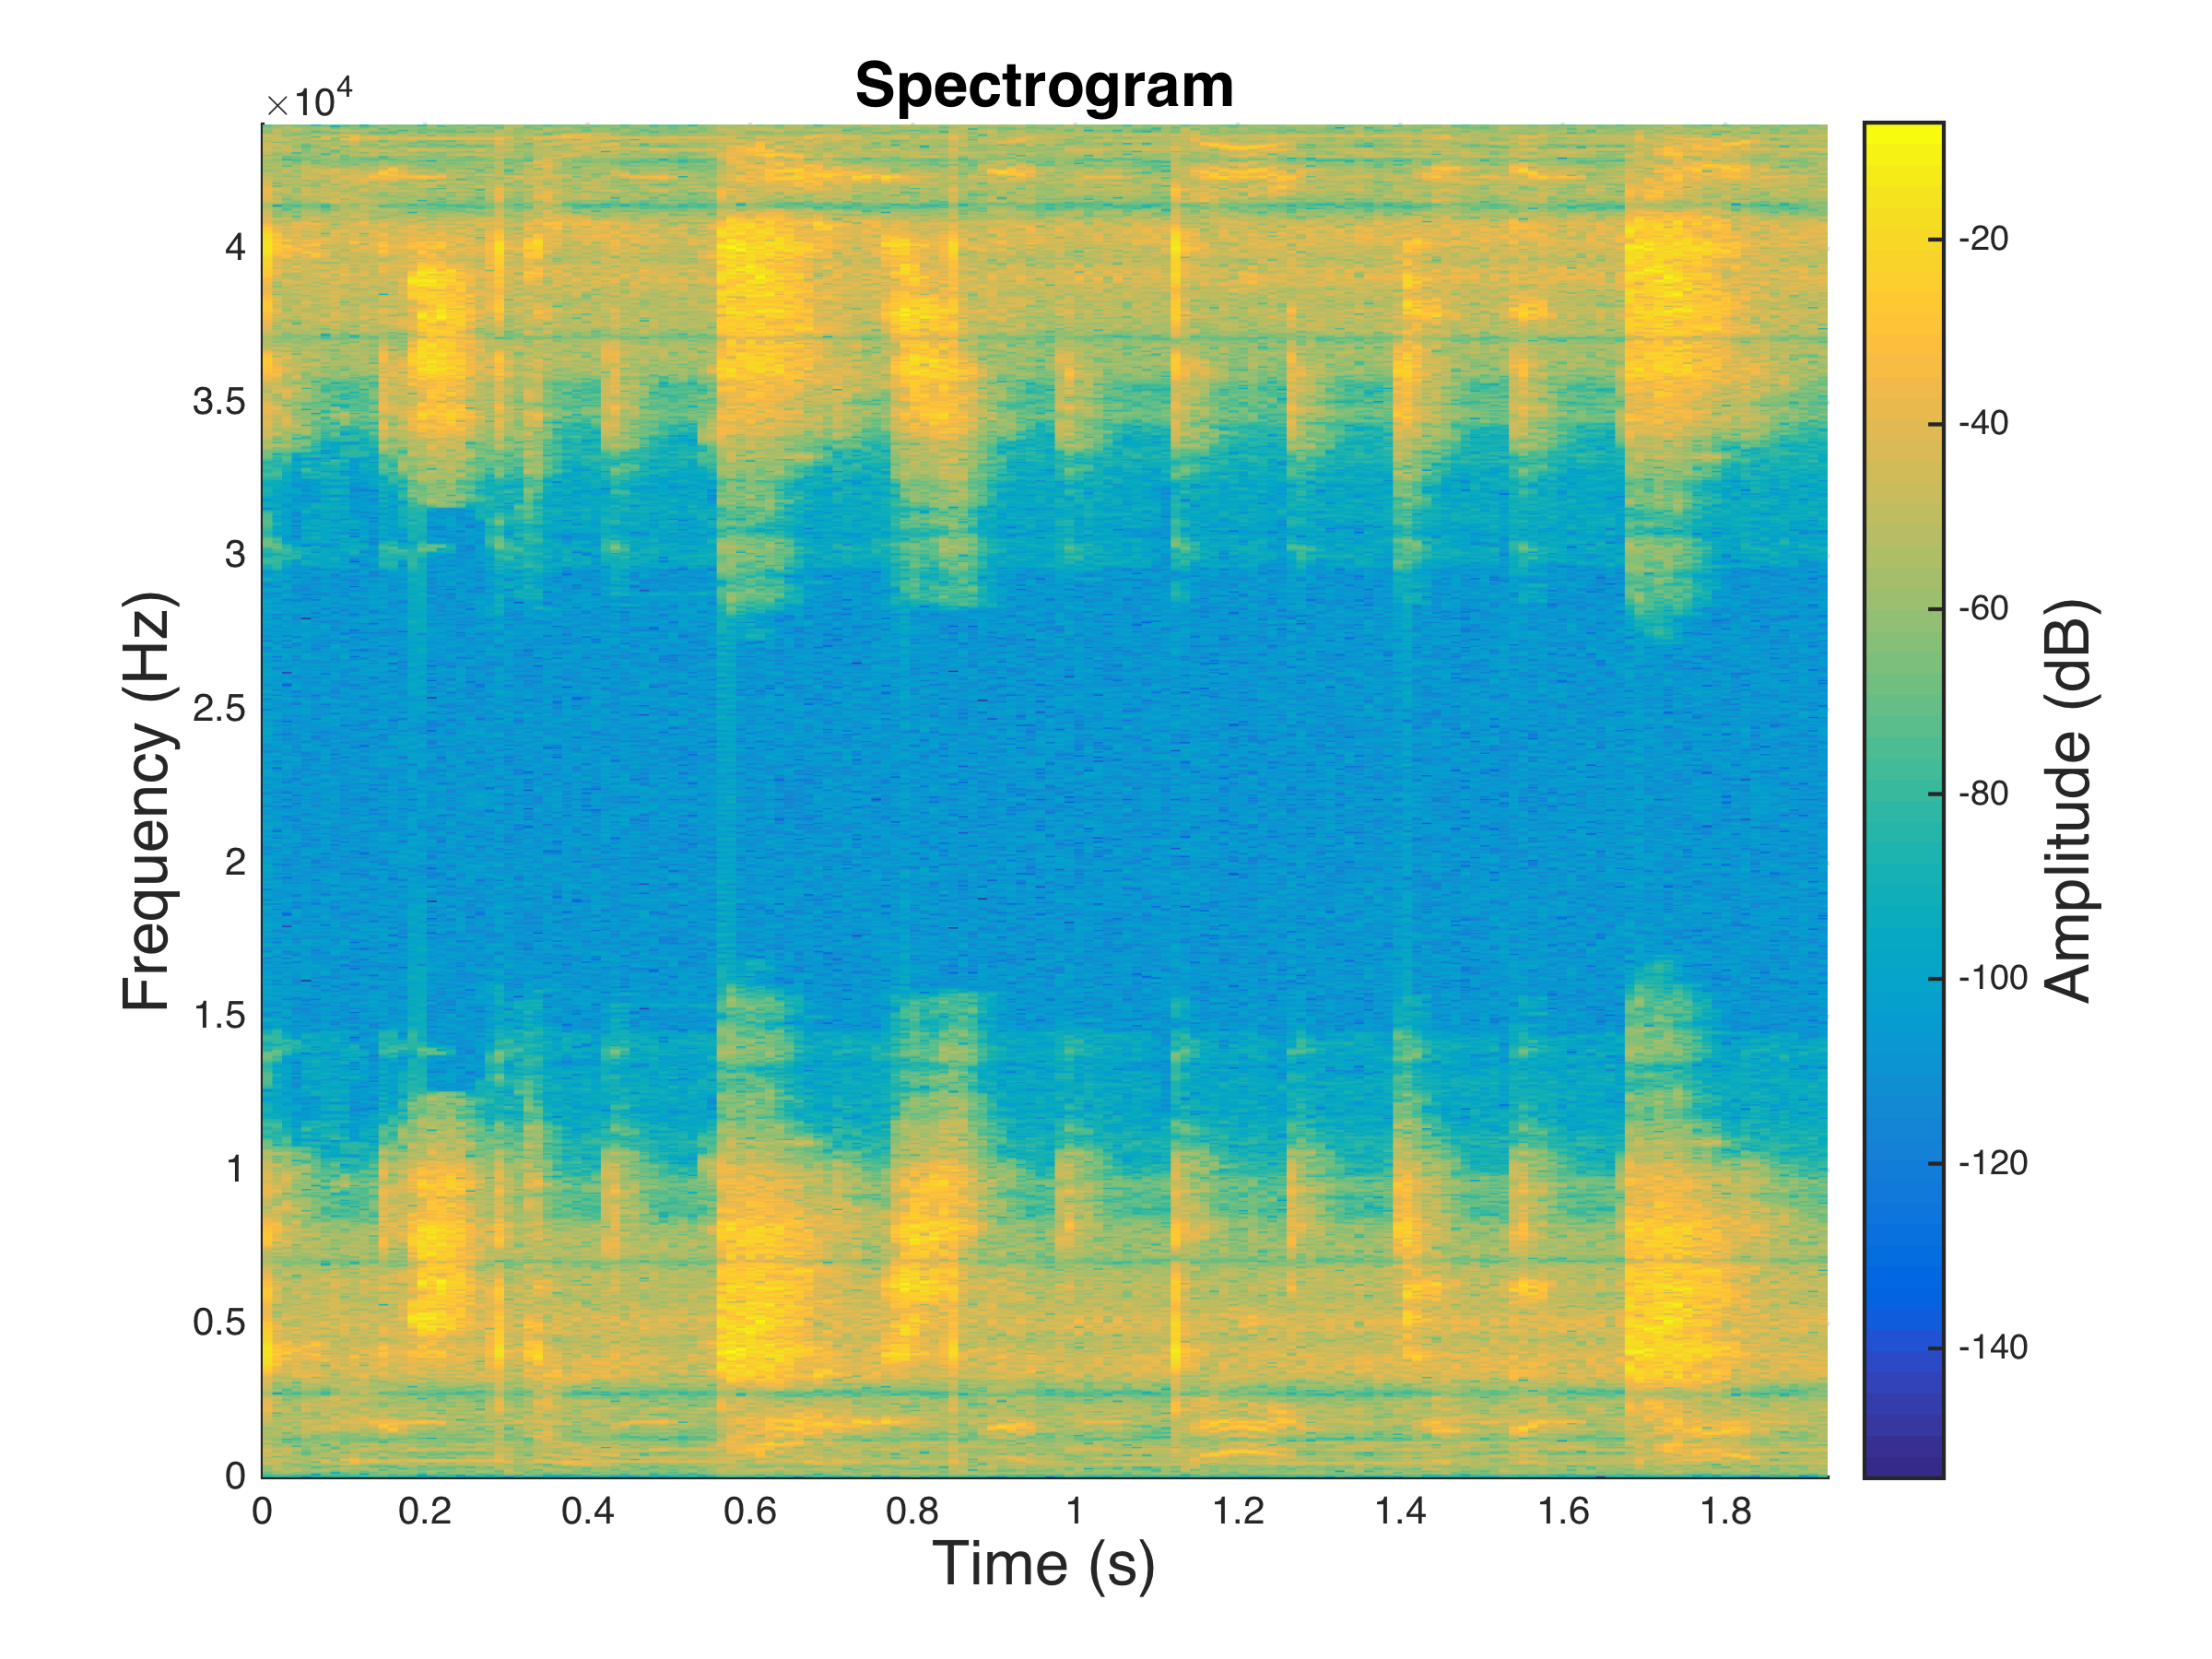
\includegraphics[scale=0.35]{music_clip1_spectrogram}
\centering
\caption{Spectrogram from random 2 second portion of Hollywood Undead song}
\centering
\end{figure}


\end{document}